\subsection*{Protein-context pharmacophore-query coverage}

\begin{figure}[htbp]
\centering
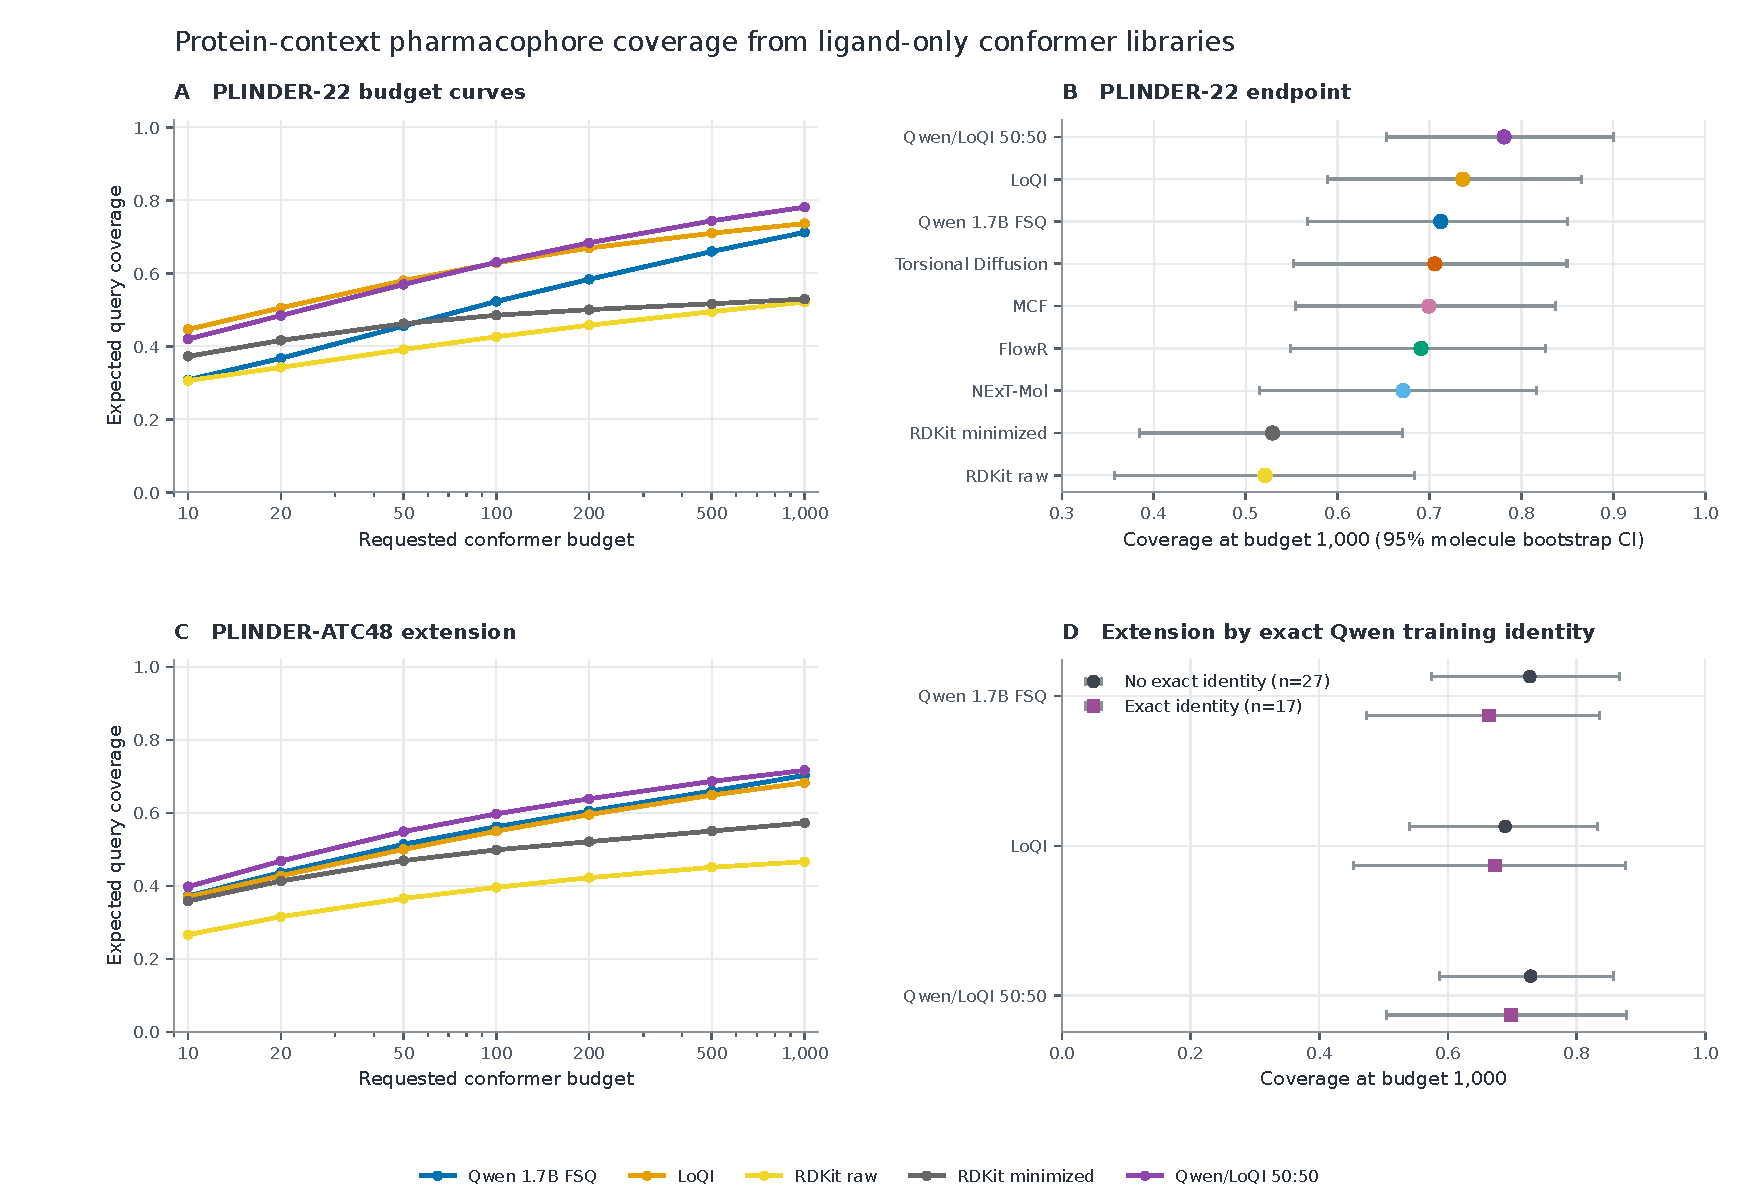
\includegraphics[width=\linewidth]{figures/supporting/pharmacophore-query-coverage.pdf}
\caption{Coverage of positional protein-contact pharmacophore queries by ligand-only
conformer libraries. (A) Expected coverage across sampling budgets in the
22-molecule PLINDER panel for Qwen, LoQI, the two RDKit pipelines, and an equal
Qwen/LoQI allocation. (B) The 1,000-conformer endpoint for the expanded method
panel; intervals resample molecules. (C) The same budget curves in the
algorithmically selected PLINDER-ATC48 extension. (D) Extension endpoints for
Qwen, LoQI, and their equal mixture, stratified by exact isomeric InChIKey identity
in the audited Qwen training export (17 eligible identities with an exact match;
27 without). All panels require every query center to match within 0.5 \AA{}, use
exact uniform sampling without replacement, average queries within molecule and
then weight molecules equally. Requested budgets are capped at supplied pool size.
The exact-identity strata are descriptive and do not exclude scaffold or
near-neighbor overlap.}
\label{fig:pharmacophore-query}
\end{figure}

The primary curves use the supplied conformer pools. In the validity sensitivity,
PoseBusters failures retain their candidate positions, consume sampling budget,
and cannot match; no post-gate replenishment is performed. Candidate-level match
membership was complete and monotone as positional tolerances increased. The
archived agreement analysis separately classifies candidates that satisfy the
0.5 \AA{} pharmacophore query, the 0.75 \AA{} whole-molecule RMSD criterion, both,
or neither after verifying candidate and reference correspondence.
